\section*{Compact Muon Solenoid}

The Compact Muon Solenoid (CMS) experiment is a general-purpose detector designed to measure the properties of all particles produced in collisions at the LHC. The CMS detector has a cylindrical layout with a central "barrel" part and two "endcap" parts at the end of either side of the barrel. The detector consists of multiple layers of sub-detectors that work together to detect and measure the various particles produced in the collisions. The sub-detectors in the CMS detector include a silicon pixel detector, a silicon strip tracker, an electromagnetic calorimeter (ECAL), a hadron calorimeter (HCAL), a superconducting solenoid, and a muon detector. Each of these sub-detectors is specialised to detect specific types of particles and measure their properties.\\
\begin{wrapfigure}{r}{0.53\textwidth}
    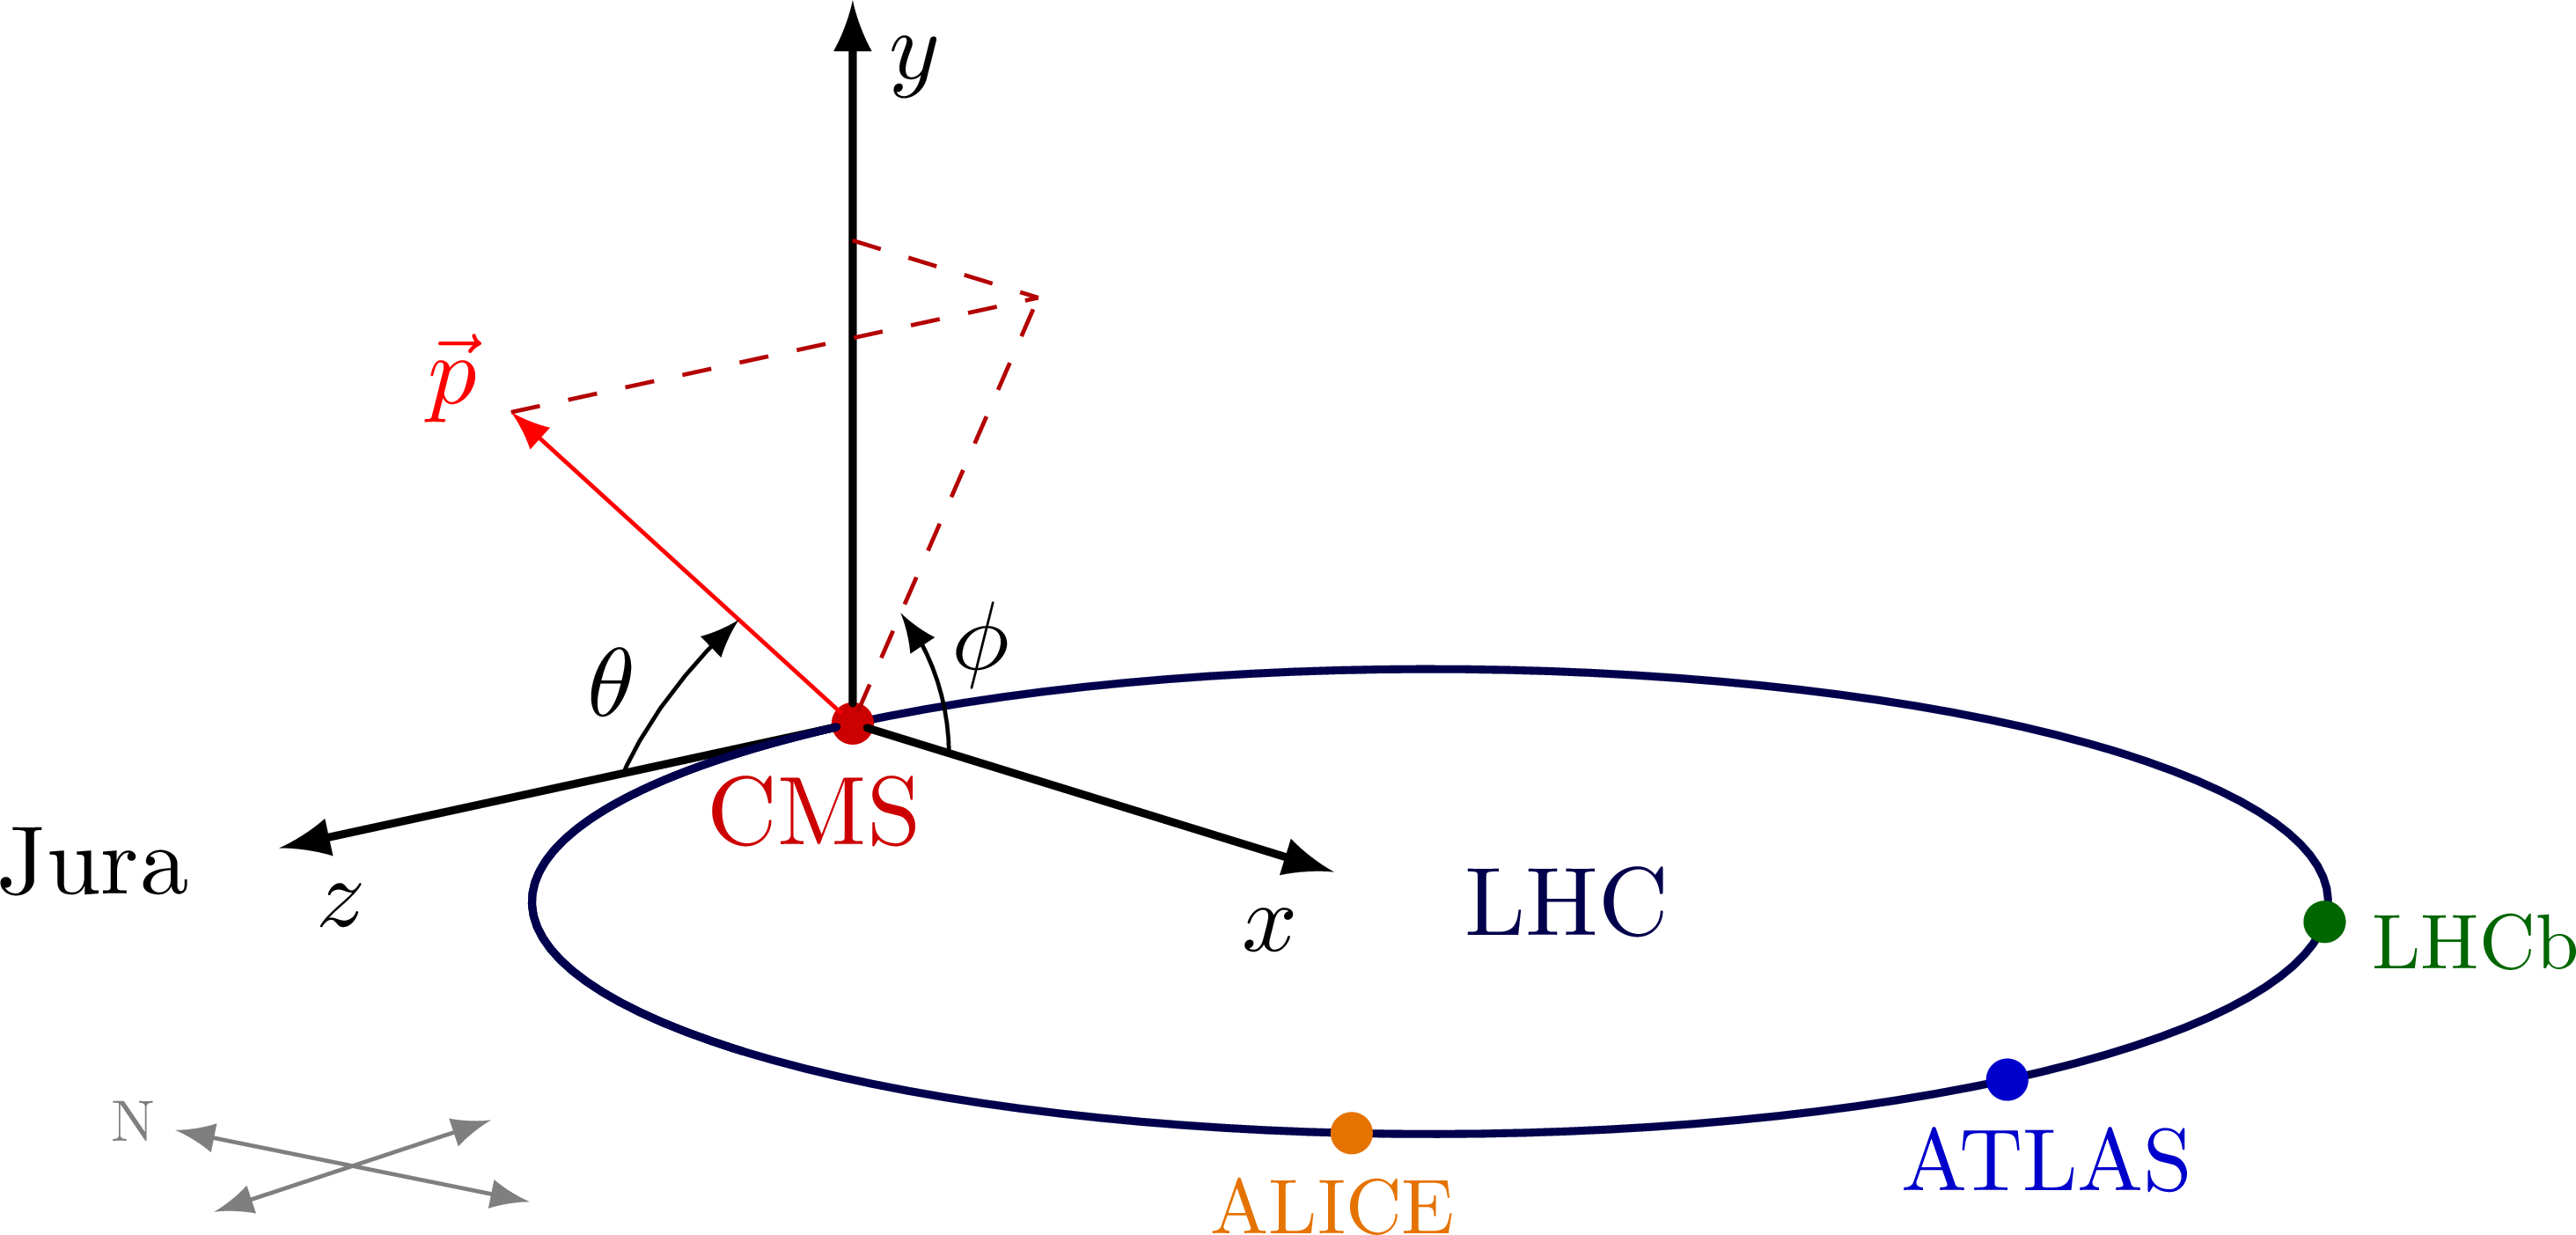
\includegraphics[width=0.53\textwidth]{CMScoordinate.png}
    \caption{CMS coordinate system, including the LHC and a compass\cite{TikZ}}
    \label{Fig:CMScoordinates}
\end{wrapfigure}
The CMS detector has adopted a coordinate system where the origin is centered at  nominal collision point
inside the experiment, The y-axis of the CMS coordinate system points vertically upward, and the x-axis points radially inward toward the center of the LHC. Thus, the z-axis points along the beam direction. The coordinates of a detected particle in the CMS experiment are defined by their azimuthal angle $\phi$ of a particle in the detector measured from the x-axis in the x-y plane, and the polar angle $\theta$ measured from the z-axis \cite{TheCMSCollaboration_2008}. a more commonly used spatial coordinate for a particle is pseudorapidity $\eta = -\ln(\tan(\theta/2))$ to represent the angle of a particle relative to the beam axis. Last, the momentum and energy transverse to the beam axis denoted by $p_T$ and $E_T$ respectively are calculated from the x and y components.

The CMS detector is capable of measuring a subset of particles of the SM, including electrons, muons (including their antiparticles), photons, and neutral and charged hadrons. When particles are generated from the interaction region, they first pass through the tracker. The tracker is responsible for measuring the trajectories of charged particles. These trajectories are influenced in the transverse direction of the beam line by the encompassing magnetic field, causing the particles track to curve. Reconstruction of particle trajectories gives a measurement for the transverse momentum $p_T$ and pseudorapidity $\eta$ of the charged particle. Within the ECAL both electrons and photons interact  repeatedly with the material resulting in the emission of a cascade of secondary particles (electromagnetic showering) until the shower reaches its maximum development. the ECAL can accurately measure the energy deposited by the electromagnetic shower to determine the primary electron or photon energy. Similarly the energy of hadrons in the experiment are measured by the HCAL. Muons are neither stopped by the ECAL or HCAL and traverse reach up to the muon chambers. In the muon chambers, the trajectories of muons are measured, providing information about their momentum and energy.

The layers of sub-detectors of the CMS detector require characteristics that optimise the measurement of a subset of particles. In addition, thousands of particles traverse the inner sub-detectors per bunch crossing requiring dedicated detector materials to support fast response. The properties of the sub-detectors are summarised in the following.
\begin{figure}[t]
    \includegraphics[width=1.0\textwidth]{CMS.png}
    \caption{A perspective view of the CMS detector}
    \label{Fig:CMS}
\end{figure}